

%To run this example in the browser through MindQuantum, follow the link:

%\href{https://blog.csdn.net/fisherish/article/details/105115272}{https://blog.csdn.net/fisherish/article/details/105115272}
%\cite{PhysRevLett.131.030402}
查看本节演示代码：\democode{05}{5.2_Quantum_Approximate_Optimization_Algorithm} \ \democodegithub{05}{5.2_Quantum_Approximate_Optimization_Algorithm}

\subsubsection{背景}

本节介绍量子近似优化算法（Quantum Approximate Optimization Algorithm, QAOA），并展示如何使用 \MindQuantum\ 实现该算法。此外，我们将在 D 节探索高级应用，在那里会应用 STA 技术实现收敛性更好的 ansatz DC-QAOA \cite{PhysRevResearch.4.013141}。


QAOA 是一种强大的量子算法，旨在利用量子计算机能力处理组合优化问题。该算法最早由 Farhi 等人在 2014 年提出 \cite{farhi2014quantum}；此后，人们发展出大量变体，用于克服原始算法的局限。

受量子绝热算法 Trotter 化版本的启发，QAOA 被归类为变分量子算法。传统 QAOA 由两个主要部分组成：量子部分涉及一个参数化线路 ansatz，经典部分负责优化这些参数。为了有效使用 QAOA 算法，我们将问题定义为寻找问题哈密顿量的基态。ansatz 由两个基本构件构成，即混合层和问题层：

\begin{equation}
    U(\gamma, \beta) = \prod_{l=1}^p e^{-i\beta_l \hat{H}_{m}}e^{-i\gamma_l\hat{H}{{p}}},
\end{equation}
其中，$\hat{H}_{{m}} = \sum_i \hat{\sigma}^x_i$ 表示混合哈密顿量，$\hat{\sigma}^x$ 对应 Pauli $x$ 算符；另一方面，$\hat{H}_{{p}}$ 表示问题哈密顿量。

量子态从 $\hat{H}_{\text{mixer}}$ 的基态开始，即 $|\psi_0\rangle=|+\rangle^{\otimes n}$。随后，QAOA ansatz 的量子态表示为：
\begin{equation}
    |\psi_p(\gamma, \beta)\rangle = e^{-i\beta_p\hat{H}_m}e^{-i\gamma_p\hat{H}_p}\cdots e^{-i\beta_1\hat{H}_{m}}e^{-i\gamma_1\hat{H}_{p}}|\psi_0\rangle.
\end{equation}
为了确定代价函数或目标函数，需要计算问题哈密顿量 $\hat{H}_{\text{prob}}$ 在 ansatz 态 $|\psi_p(\gamma, \beta)\rangle$ 上的期望值。这涉及在计算基下对最终态进行重复测量：
\begin{equation}
    F_p(\gamma, \beta) =\langle\psi_p(\gamma, \beta)|\hat{H}_{p} |\psi_p(\gamma,\beta)\rangle.
\end{equation}
QAOA 的主要目标是找到使期望值 $F_p(\gamma, \beta)$ 最小的最优参数 $(\gamma^*, \beta^*)$。实现这一目标需要使用经典优化算法迭代更新参数 $\gamma$ 和 $\beta$：
\begin{equation}
    (\gamma^*, \beta^*) = \text{arg}\min_{\gamma, \beta} F_p(\gamma, \beta).
\end{equation}

通过寻找这些最优参数，QAOA 使量子计算机能够高效应对复杂优化挑战，并为多种实际应用提供了有前景的途径。




\subsubsection{实现}

在本教程中，我们使用 QAOA 算法处理最大割问题，这是图论中的一个 NP 完全问题。如图 \ref{5.1_QAOA} 所示，该问题需要将图的顶点划分为两部分，并使被切割的边数量最大化。但当图中顶点数量增加时，很难找到有效的经典算法来求解最大割问题，因为这类 NP 完全问题很可能不存在多项式时间算法。

\begin{figure}[H]
    \centering
    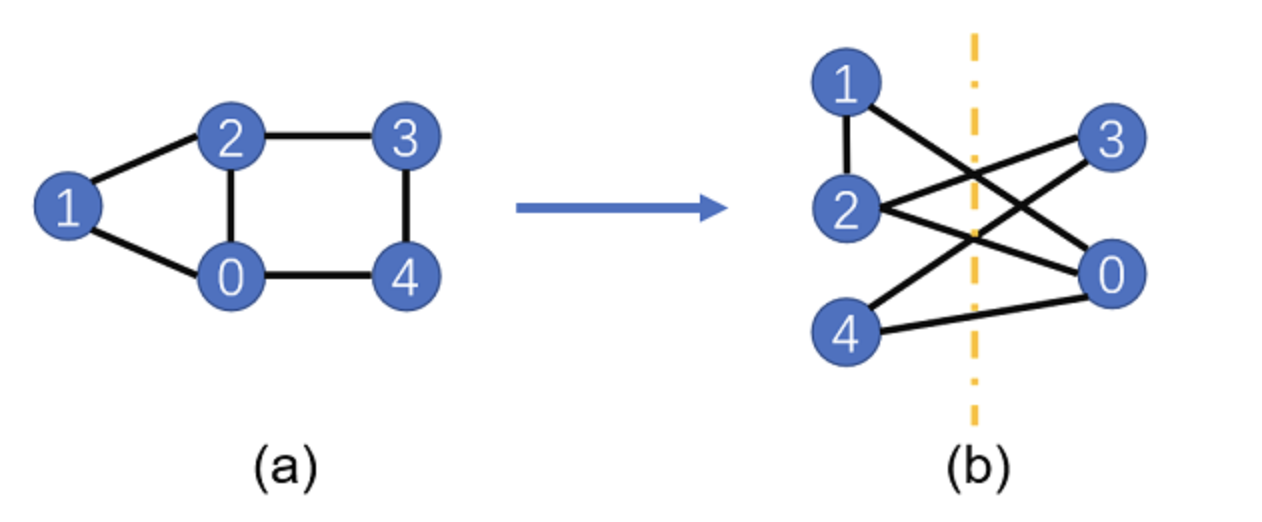
\includegraphics[width=0.49\textwidth]{5.2_figures/5.2_QAOA}
    \caption{最大割图}
    \label{5.1_QAOA}
\end{figure}

首先使用 \textit{NetworkX} \cite{SciPyProceedings_11} 生成一个由五个顶点和六条边组成的图结构。
\begin{lstlisting}
g = nx.Graph()
nx.add_path(g, [0,1])
nx.add_path(g, [1,2])
nx.add_path(g, [2,3])
nx.add_path(g, [3,4])
nx.add_path(g, [0,4])
nx.add_path(g, [0,2])
nx.draw(g,with_labels=True, font_weight='bold')
\end{lstlisting}

对于 QAOA 算法，首先需要将最大割问题转换为哈密顿量，其基态能量对应问题的解。最大割问题的问题哈密顿量可以构造为
\begin{equation}
    \hat{H} = \sum_{(i,j)\in C}(\hat{Z}_i\hat{Z}_j-1)/2,
\end{equation}
其中 $C$ 是所有边的集合。在下面的函数 \code{build\_ham} 中，可以通过输入图来构造对应哈密顿量。
\begin{lstlisting}
def build_ham(g):
    hc = QubitOperator()
    for i in g.edges:
        hc += QubitOperator(f'Z{i[0]} Z{i[1]}')
    return hc
\end{lstlisting}
接下来构造 QAOA ansatz，其中函数 \code{build\_hc} 和 \code{build\_hb} 分别根据问题哈密顿量和混合哈密顿量构造量子线路。通过向函数 \code{build\_ansatz} 输入图，可以直接构建 ansatz。

\begin{lstlisting}
def build_hc(g,para):
    hc = Circuit()
    for i in g.edges:
        hc += Rzz(para).on(i)
    return hc
def build_hb(g, para):
    hc = Circuit()
    for i in g.nodes:
        hc += RX(para).on(i)
    return hc
def build_ansatz(g, p):
    c = Circuit()
    for i in range(p):
        c += build_hc(g,f'g{i}')
        c += build_hb(g,f'b{i}')
    return c
\end{lstlisting}

在本例中选择 $p=4$，表示使用四层 QAOA 量子线路。\code{init\_state\_circ} 是用于将初态制备为均匀叠加态的量子线路。
\begin{lstlisting}
p = 4
ham = Hamiltonian(build_ham(g))
ansatz = build_ansatz(g, p)
init_state_circ = UN(H, g.nodes)
\end{lstlisting}

QAOA 的目标是找到最优参数，使代价函数或哈密顿量期望值 $\mathcal{E}=\langle \psi(\gamma, \beta)|\hat{H}|\psi(\gamma, \beta)\rangle$ 最小。
该问题不需要编码层量子线路，因此我们使用 \MQAnsatzOnlyLayer\ 作为待训练的量子神经网络，并使用 Adam 作为优化器。
\begin{lstlisting}
import mindspore as ms
ms.set_context(mode=ms.PYNATIVE_MODE, device_target="CPU")

total_circuit = init_state_circ + ansatz
sim = Simulator('mqvector', total_circuit.n_qubits)
grad_ops = sim.get_expectation_with_grad(ham, total_circuit)
net = MQAnsatzOnlyLayer(grad_ops)
opti = nn.Adam(net.trainable_params(), learning_rate=0.05)
train_net = nn.TrainOneStepCell(net, opti)

for i in range(600):
    if i%10 == 0:
        print("train step:", i, ", cut:", (len(g.edges)-train_net())/2)
\end{lstlisting}
\begin{lstlisting}
train step: 0 ,   cut: [3.0001478]
train step: 10 ,  cut: [4.1718774]
train step: 20 ,  cut: [4.6871986]
train step: 30 ,  cut: [4.7258005]
train step: 40 ,  cut: [4.804503]
train step: 50 ,  cut: [4.8477592]
train step: 60 ,  cut: [4.8705964]
train step: 70 ,  cut: [4.9060946]
train step: 80 ,  cut: [4.933446]
train step: 90 ,  cut: [4.9356637]
train step: 100 , cut: [4.938308]
train step: 110 , cut: [4.9390197]
train step: 120 , cut: [4.939068]
train step: 130 , cut: [4.9392157]
train step: 140 , cut: [4.939249]
train step: 150 , cut: [4.939247]
train step: 160 , cut: [4.939255]
train step: 170 , cut: [4.939257]
train step: 180 , cut: [4.939257]
train step: 190 , cut: [4.939257]
\end{lstlisting}

根据上述训练结果可以发现，该问题哈密顿量基态能量对应的割边数量接近 5。

在 \MindQuantum\ 中，可以直接导入 \MaxCutAnsatz\ 函数来构建最大割问题的 ansatz。
\begin{lstlisting}
import numpy as np
from mindquantum.algorithm.nisq import MaxCutAnsatz
graph = [(0, 1), (1, 2), (0, 2)]
p = 1 # 层数
maxcut = MaxCutAnsatz(graph, p)
maxcut.circuit.svg()
\end{lstlisting}
\begin{figure}[H]
    \centering
    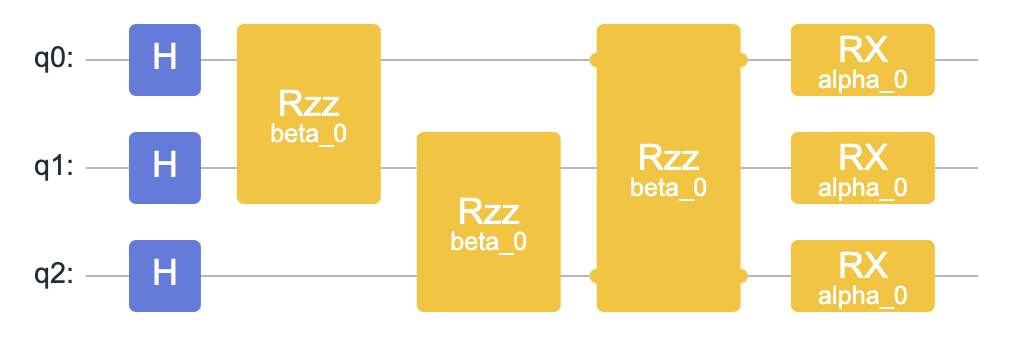
\includegraphics[width=0.49\textwidth]{5.2_figures/5.2_QAOA_ansatze}
    \caption{最大割问题 Ansatz}
    \label{5.1_QAOA_ansatz}
\end{figure}
同时，也可以获得哈密顿量：
\begin{lstlisting}
print(maxcut.hamiltonian)
\end{lstlisting}
\begin{lstlisting}
3/2 [] +
-1/2 [Z0 Z1] +
-1/2 [Z1 Z2] +
-1/2 [Z0 Z2]
\end{lstlisting}
最大割问题的切割方案以及该方案中的割边数量，可以通过函数 $get\_partition$ 和 $get\_cut\_value$ 获得。切割方案是由两个列表组成的列表数组，每个列表数组都包含被切分到对应部分的节点。
\begin{lstlisting}
partitions = maxcut.get_partition(5, np.array([4, 1]))
for i in partitions:
    print(f'partition: left: {i[0]}, right: {i[1]}, cut value: {maxcut.get_cut_value(i)}')
\end{lstlisting}
\begin{lstlisting}
partition: left: [0, 2],   right: [1], cut value: 2
partition: left: [1, 2],   right: [0], cut value: 2
partition: left: [1],   right: [0, 2], cut value: 2
partition: left: [0, 1, 2], right: [], cut value: 0
partition: left: [], right: [0, 1, 2], cut value: 0
\end{lstlisting}









